\documentclass[a4paper,11pt]{article}
\usepackage[left=1.5cm,right=1.5cm,top=1.1cm,bottom=1.0cm]{geometry}
\usepackage{fontspec}
\setmainfont{Red Hat Text}[BoldFont={Red Hat Text SemiBold}]
\newfontfamily\display{Red Hat Display}[BoldFont={Red Hat Display Bold}]
\newfontfamily\mono{Red Hat Mono}[BoldFont={Red Hat Mono SemiBold}]
\usepackage{tikz}
\usepackage{graphicx}
\pagestyle{empty}
\setlength{\parindent}{0pt}

\definecolor{ink}{HTML}{1A1A1A}
\definecolor{klar}{HTML}{1F3B5B}
\definecolor{wandblau}{HTML}{1A5FB4}
\definecolor{wandrot}{HTML}{C01C28}
\definecolor{textblue}{HTML}{1F2E43}

\InputIfFileExists{fusszeile}{}{% Fußzeile der eigenen Vorlagen: Urheber, Lizenz und wo es die Datei gibt,
% als Text und QR-Code. Zieht die Webseite um, nur \webseite und
% \webseitetext ändern und die Vorlagen neu übersetzen.
% Einbinden in der Präambel mit % Fußzeile der eigenen Vorlagen: Urheber, Lizenz und wo es die Datei gibt,
% als Text und QR-Code. Zieht die Webseite um, nur \webseite und
% \webseitetext ändern und die Vorlagen neu übersetzen.
% Einbinden in der Präambel mit % Fußzeile der eigenen Vorlagen: Urheber, Lizenz und wo es die Datei gibt,
% als Text und QR-Code. Zieht die Webseite um, nur \webseite und
% \webseitetext ändern und die Vorlagen neu übersetzen.
% Einbinden in der Präambel mit \input{../fusszeile}; erwartet die Farbe
% textblue.
\usepackage{qrcode}

\newcommand{\webseite}{https://agag-rptu.github.io/KryptoWeb/Kopiervorlagen/}
\newcommand{\webseitetext}{agag-rptu.github.io/KryptoWeb/Kopiervorlagen}

\newcommand{\fusszeile}{%
  \noindent
  \begin{minipage}[c]{\dimexpr\textwidth-1.8cm\relax}
    \scriptsize\color{textblue}
    © 2026 Max Horn, RPTU Kaiserslautern-Landau · Lizenz CC BY-SA 4.0,
    creativecommons.org/licenses/by-sa/4.0/deed.de\\
    Diese und weitere Vorlagen als Datei: \textbf{\webseitetext}
  \end{minipage}\hfill
  \begin{minipage}[c]{1.4cm}
    \qrcode[height=1.4cm]{\webseite}%
  \end{minipage}%
}
; erwartet die Farbe
% textblue.
\usepackage{qrcode}

\newcommand{\webseite}{https://agag-rptu.github.io/KryptoWeb/Kopiervorlagen/}
\newcommand{\webseitetext}{agag-rptu.github.io/KryptoWeb/Kopiervorlagen}

\newcommand{\fusszeile}{%
  \noindent
  \begin{minipage}[c]{\dimexpr\textwidth-1.8cm\relax}
    \scriptsize\color{textblue}
    © 2026 Max Horn, RPTU Kaiserslautern-Landau · Lizenz CC BY-SA 4.0,
    creativecommons.org/licenses/by-sa/4.0/deed.de\\
    Diese und weitere Vorlagen als Datei: \textbf{\webseitetext}
  \end{minipage}\hfill
  \begin{minipage}[c]{1.4cm}
    \qrcode[height=1.4cm]{\webseite}%
  \end{minipage}%
}
; erwartet die Farbe
% textblue.
\usepackage{qrcode}

\newcommand{\webseite}{https://agag-rptu.github.io/KryptoWeb/Kopiervorlagen/}
\newcommand{\webseitetext}{agag-rptu.github.io/KryptoWeb/Kopiervorlagen}

\newcommand{\fusszeile}{%
  \noindent
  \begin{minipage}[c]{\dimexpr\textwidth-1.8cm\relax}
    \scriptsize\color{textblue}
    © 2026 Max Horn, RPTU Kaiserslautern-Landau · Lizenz CC BY-SA 4.0,
    creativecommons.org/licenses/by-sa/4.0/deed.de\\
    Diese und weitere Vorlagen als Datei: \textbf{\webseitetext}
  \end{minipage}\hfill
  \begin{minipage}[c]{1.4cm}
    \qrcode[height=1.4cm]{\webseite}%
  \end{minipage}%
}
}
% Fußzeile nur auf Seite 2, Seite 1 ist voll
\newcommand{\blattfuss}{\fusszeile[Vortraege/kinderuni-2026-11-18][Blatt, Folien und LaTeX-Quelle als Datei]}

\newcommand{\fs}[1]{\fontsize{#1}{#1}\selectfont}
\newcommand{\aufgabe}[2]{{\display\color{klar}\bfseries\fs{14}#1}\quad{\fs{11}#2}\par\vspace{2mm}}

\begin{document}
\color{ink}

\begin{minipage}[b]{13cm}
{\display\fs{28}\color{klar} GEHEIMBOTSCHAFTEN}\par\vspace{2.5mm}
{\display\bfseries\fs{13} Agenten-Blatt}\quad{\fs{10.5} Kinder-Uni der RPTU · 18. November 2026}
\end{minipage}\hfill

\includegraphics[height=1.55cm]{rptu-logo.pdf}\par
\vspace{3mm}
{\fs{11} Agentenname: \rule{4.5cm}{0.5pt}}\hfill{\fs{10.5} Vorlesung von \textbf{Prof. Dr. Max Horn}, Fachbereich Mathematik}\par
\vspace{3.5mm}

\begin{minipage}[t]{7.6cm}\vspace{0pt}
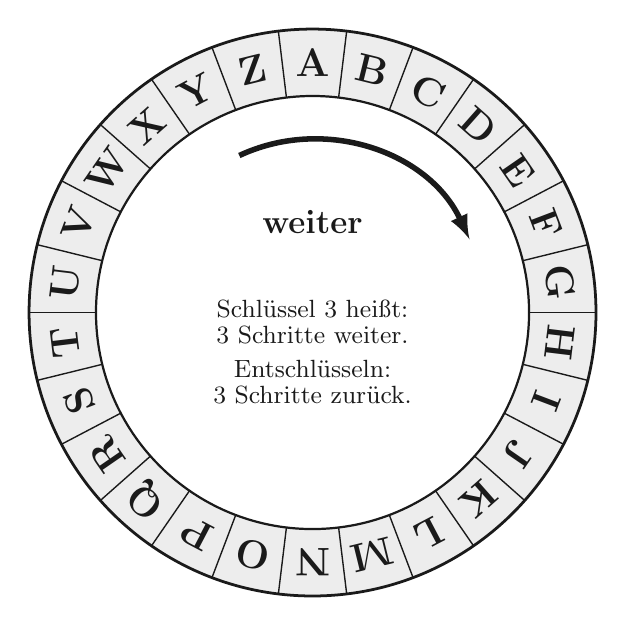
\begin{tikzpicture}
\draw[ink, fill=black!7, line width=1pt] (0,0) circle (3.6);
\draw[ink, fill=white, line width=0.8pt] (0,0) circle (2.75);
\draw[ink, line width=0.5pt] (83.07692307692308:2.75) -- (83.07692307692308:3.6);
\node[font=\bfseries\fs{14}, text=ink, rotate=0.0] at (90.0:3.17) {A};
\draw[ink, line width=0.5pt] (69.23076923076923:2.75) -- (69.23076923076923:3.6);
\node[font=\bfseries\fs{14}, text=ink, rotate=-13.84615384615384] at (76.15384615384616:3.17) {B};
\draw[ink, line width=0.5pt] (55.38461538461539:2.75) -- (55.38461538461539:3.6);
\node[font=\bfseries\fs{14}, text=ink, rotate=-27.692307692307693] at (62.30769230769231:3.17) {C};
\draw[ink, line width=0.5pt] (41.53846153846154:2.75) -- (41.53846153846154:3.6);
\node[font=\bfseries\fs{14}, text=ink, rotate=-41.53846153846154] at (48.46153846153846:3.17) {D};
\draw[ink, line width=0.5pt] (27.692307692307693:2.75) -- (27.692307692307693:3.6);
\node[font=\bfseries\fs{14}, text=ink, rotate=-55.38461538461539] at (34.61538461538461:3.17) {E};
\draw[ink, line width=0.5pt] (13.84615384615384:2.75) -- (13.84615384615384:3.6);
\node[font=\bfseries\fs{14}, text=ink, rotate=-69.23076923076923] at (20.769230769230774:3.17) {F};
\draw[ink, line width=0.5pt] (0.0:2.75) -- (0.0:3.6);
\node[font=\bfseries\fs{14}, text=ink, rotate=-83.07692307692308] at (6.92307692307692:3.17) {G};
\draw[ink, line width=0.5pt] (-13.84615384615384:2.75) -- (-13.84615384615384:3.6);
\node[font=\bfseries\fs{14}, text=ink, rotate=-96.92307692307692] at (-6.92307692307692:3.17) {H};
\draw[ink, line width=0.5pt] (-27.692307692307693:2.75) -- (-27.692307692307693:3.6);
\node[font=\bfseries\fs{14}, text=ink, rotate=-110.76923076923077] at (-20.769230769230774:3.17) {I};
\draw[ink, line width=0.5pt] (-41.53846153846155:2.75) -- (-41.53846153846155:3.6);
\node[font=\bfseries\fs{14}, text=ink, rotate=-124.61538461538461] at (-34.61538461538461:3.17) {J};
\draw[ink, line width=0.5pt] (-55.38461538461539:2.75) -- (-55.38461538461539:3.6);
\node[font=\bfseries\fs{14}, text=ink, rotate=-138.46153846153845] at (-48.46153846153845:3.17) {K};
\draw[ink, line width=0.5pt] (-69.23076923076923:2.75) -- (-69.23076923076923:3.6);
\node[font=\bfseries\fs{14}, text=ink, rotate=-152.30769230769232] at (-62.30769230769232:3.17) {L};
\draw[ink, line width=0.5pt] (-83.07692307692307:2.75) -- (-83.07692307692307:3.6);
\node[font=\bfseries\fs{14}, text=ink, rotate=-166.15384615384616] at (-76.15384615384616:3.17) {M};
\draw[ink, line width=0.5pt] (-96.92307692307693:2.75) -- (-96.92307692307693:3.6);
\node[font=\bfseries\fs{14}, text=ink, rotate=-180.0] at (-90.0:3.17) {N};
\draw[ink, line width=0.5pt] (-110.76923076923077:2.75) -- (-110.76923076923077:3.6);
\node[font=\bfseries\fs{14}, text=ink, rotate=-193.84615384615384] at (-103.84615384615384:3.17) {O};
\draw[ink, line width=0.5pt] (-124.61538461538461:2.75) -- (-124.61538461538461:3.6);
\node[font=\bfseries\fs{14}, text=ink, rotate=-207.69230769230768] at (-117.69230769230768:3.17) {P};
\draw[ink, line width=0.5pt] (-138.46153846153845:2.75) -- (-138.46153846153845:3.6);
\node[font=\bfseries\fs{14}, text=ink, rotate=-221.53846153846155] at (-131.53846153846155:3.17) {Q};
\draw[ink, line width=0.5pt] (-152.30769230769232:2.75) -- (-152.30769230769232:3.6);
\node[font=\bfseries\fs{14}, text=ink, rotate=-235.3846153846154] at (-145.3846153846154:3.17) {R};
\draw[ink, line width=0.5pt] (-166.15384615384613:2.75) -- (-166.15384615384613:3.6);
\node[font=\bfseries\fs{14}, text=ink, rotate=-249.23076923076923] at (-159.23076923076923:3.17) {S};
\draw[ink, line width=0.5pt] (-180.0:2.75) -- (-180.0:3.6);
\node[font=\bfseries\fs{14}, text=ink, rotate=-263.0769230769231] at (-173.0769230769231:3.17) {T};
\draw[ink, line width=0.5pt] (-193.84615384615387:2.75) -- (-193.84615384615387:3.6);
\node[font=\bfseries\fs{14}, text=ink, rotate=-276.9230769230769] at (-186.9230769230769:3.17) {U};
\draw[ink, line width=0.5pt] (-207.69230769230768:2.75) -- (-207.69230769230768:3.6);
\node[font=\bfseries\fs{14}, text=ink, rotate=-290.7692307692308] at (-200.76923076923077:3.17) {V};
\draw[ink, line width=0.5pt] (-221.53846153846155:2.75) -- (-221.53846153846155:3.6);
\node[font=\bfseries\fs{14}, text=ink, rotate=-304.61538461538464] at (-214.61538461538464:3.17) {W};
\draw[ink, line width=0.5pt] (-235.38461538461536:2.75) -- (-235.38461538461536:3.6);
\node[font=\bfseries\fs{14}, text=ink, rotate=-318.46153846153845] at (-228.46153846153845:3.17) {X};
\draw[ink, line width=0.5pt] (-249.23076923076923:2.75) -- (-249.23076923076923:3.6);
\node[font=\bfseries\fs{14}, text=ink, rotate=-332.3076923076923] at (-242.30769230769232:3.17) {Y};
\draw[ink, line width=0.5pt] (-263.0769230769231:2.75) -- (-263.0769230769231:3.6);
\node[font=\bfseries\fs{14}, text=ink, rotate=-346.15384615384613] at (-256.15384615384613:3.17) {Z};
\draw[ink, line width=2pt, -latex] (115:2.2) arc (115:25:2.2);
\node[font=\bfseries\fs{12}, text=ink] at (0,1.15) {weiter};
\node[font=\fs{9.5}, text=ink, align=center] at (0,-0.5) {Schlüssel 3 heißt:\\3 Schritte weiter.\\[1mm]Entschlüsseln:\\3 Schritte zurück.};
\end{tikzpicture}
\end{minipage}\hfill
\begin{minipage}[t]{9.8cm}\vspace{0pt}
\aufgabe{1 · Dein Name wird geheim}{}
{\fs{11} Wähle einen Schlüssel von 1 bis 6: \rule{1.2cm}{0.5pt}}\par\vspace{2.5mm}
{\fs{11} Dein Vorname, verschlüsselt:}\par\vspace{1mm}
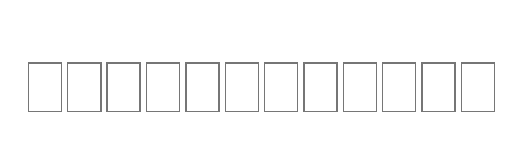
\begin{tikzpicture}
\node[font=\mono\bfseries\fs{13}, text=ink] at (0.25,0.95) {};
\draw[ink!60, line width=0.5pt] (0.04,0) rectangle (0.46,0.62);
\node[font=\mono\bfseries\fs{13}, text=ink] at (0.75,0.95) {};
\draw[ink!60, line width=0.5pt] (0.54,0) rectangle (0.96,0.62);
\node[font=\mono\bfseries\fs{13}, text=ink] at (1.25,0.95) {};
\draw[ink!60, line width=0.5pt] (1.04,0) rectangle (1.46,0.62);
\node[font=\mono\bfseries\fs{13}, text=ink] at (1.75,0.95) {};
\draw[ink!60, line width=0.5pt] (1.54,0) rectangle (1.96,0.62);
\node[font=\mono\bfseries\fs{13}, text=ink] at (2.25,0.95) {};
\draw[ink!60, line width=0.5pt] (2.04,0) rectangle (2.46,0.62);
\node[font=\mono\bfseries\fs{13}, text=ink] at (2.75,0.95) {};
\draw[ink!60, line width=0.5pt] (2.54,0) rectangle (2.96,0.62);
\node[font=\mono\bfseries\fs{13}, text=ink] at (3.25,0.95) {};
\draw[ink!60, line width=0.5pt] (3.04,0) rectangle (3.46,0.62);
\node[font=\mono\bfseries\fs{13}, text=ink] at (3.75,0.95) {};
\draw[ink!60, line width=0.5pt] (3.54,0) rectangle (3.96,0.62);
\node[font=\mono\bfseries\fs{13}, text=ink] at (4.25,0.95) {};
\draw[ink!60, line width=0.5pt] (4.04,0) rectangle (4.46,0.62);
\node[font=\mono\bfseries\fs{13}, text=ink] at (4.75,0.95) {};
\draw[ink!60, line width=0.5pt] (4.54,0) rectangle (4.96,0.62);
\node[font=\mono\bfseries\fs{13}, text=ink] at (5.25,0.95) {};
\draw[ink!60, line width=0.5pt] (5.04,0) rectangle (5.46,0.62);
\node[font=\mono\bfseries\fs{13}, text=ink] at (5.75,0.95) {};
\draw[ink!60, line width=0.5pt] (5.54,0) rectangle (5.96,0.62);
\end{tikzpicture}\par\vspace{2.5mm}
{\fs{11} Tausche das Blatt mit deinem Nachbarn. Entschlüsselt:}\par\vspace{1mm}
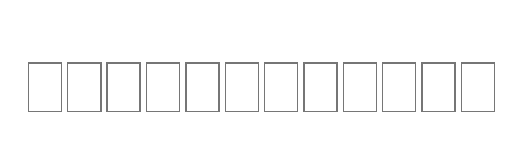
\begin{tikzpicture}
\node[font=\mono\bfseries\fs{13}, text=ink] at (0.25,0.95) {};
\draw[ink!60, line width=0.5pt] (0.04,0) rectangle (0.46,0.62);
\node[font=\mono\bfseries\fs{13}, text=ink] at (0.75,0.95) {};
\draw[ink!60, line width=0.5pt] (0.54,0) rectangle (0.96,0.62);
\node[font=\mono\bfseries\fs{13}, text=ink] at (1.25,0.95) {};
\draw[ink!60, line width=0.5pt] (1.04,0) rectangle (1.46,0.62);
\node[font=\mono\bfseries\fs{13}, text=ink] at (1.75,0.95) {};
\draw[ink!60, line width=0.5pt] (1.54,0) rectangle (1.96,0.62);
\node[font=\mono\bfseries\fs{13}, text=ink] at (2.25,0.95) {};
\draw[ink!60, line width=0.5pt] (2.04,0) rectangle (2.46,0.62);
\node[font=\mono\bfseries\fs{13}, text=ink] at (2.75,0.95) {};
\draw[ink!60, line width=0.5pt] (2.54,0) rectangle (2.96,0.62);
\node[font=\mono\bfseries\fs{13}, text=ink] at (3.25,0.95) {};
\draw[ink!60, line width=0.5pt] (3.04,0) rectangle (3.46,0.62);
\node[font=\mono\bfseries\fs{13}, text=ink] at (3.75,0.95) {};
\draw[ink!60, line width=0.5pt] (3.54,0) rectangle (3.96,0.62);
\node[font=\mono\bfseries\fs{13}, text=ink] at (4.25,0.95) {};
\draw[ink!60, line width=0.5pt] (4.04,0) rectangle (4.46,0.62);
\node[font=\mono\bfseries\fs{13}, text=ink] at (4.75,0.95) {};
\draw[ink!60, line width=0.5pt] (4.54,0) rectangle (4.96,0.62);
\node[font=\mono\bfseries\fs{13}, text=ink] at (5.25,0.95) {};
\draw[ink!60, line width=0.5pt] (5.04,0) rectangle (5.46,0.62);
\node[font=\mono\bfseries\fs{13}, text=ink] at (5.75,0.95) {};
\draw[ink!60, line width=0.5pt] (5.54,0) rectangle (5.96,0.62);
\end{tikzpicture}\par
\vspace{3.5mm}
\aufgabe{2 · Mini-Quiz}{Schlüssel 3}
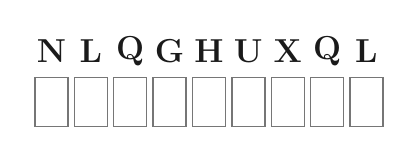
\begin{tikzpicture}
\node[font=\mono\bfseries\fs{13}, text=ink] at (0.25,0.95) {N};
\draw[ink!60, line width=0.5pt] (0.04,0) rectangle (0.46,0.62);
\node[font=\mono\bfseries\fs{13}, text=ink] at (0.75,0.95) {L};
\draw[ink!60, line width=0.5pt] (0.54,0) rectangle (0.96,0.62);
\node[font=\mono\bfseries\fs{13}, text=ink] at (1.25,0.95) {Q};
\draw[ink!60, line width=0.5pt] (1.04,0) rectangle (1.46,0.62);
\node[font=\mono\bfseries\fs{13}, text=ink] at (1.75,0.95) {G};
\draw[ink!60, line width=0.5pt] (1.54,0) rectangle (1.96,0.62);
\node[font=\mono\bfseries\fs{13}, text=ink] at (2.25,0.95) {H};
\draw[ink!60, line width=0.5pt] (2.04,0) rectangle (2.46,0.62);
\node[font=\mono\bfseries\fs{13}, text=ink] at (2.75,0.95) {U};
\draw[ink!60, line width=0.5pt] (2.54,0) rectangle (2.96,0.62);
\node[font=\mono\bfseries\fs{13}, text=ink] at (3.25,0.95) {X};
\draw[ink!60, line width=0.5pt] (3.04,0) rectangle (3.46,0.62);
\node[font=\mono\bfseries\fs{13}, text=ink] at (3.75,0.95) {Q};
\draw[ink!60, line width=0.5pt] (3.54,0) rectangle (3.96,0.62);
\node[font=\mono\bfseries\fs{13}, text=ink] at (4.25,0.95) {L};
\draw[ink!60, line width=0.5pt] (4.04,0) rectangle (4.46,0.62);
\end{tikzpicture}
\end{minipage}\par
\vspace{3.5mm}

\aufgabe{3 · Abgefangen!}{Der Schlüssel ist unbekannt. Probiert es am ersten Wort aus.}
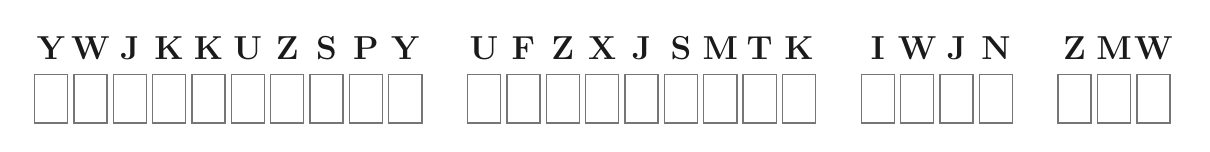
\begin{tikzpicture}
\node[font=\mono\bfseries\fs{13}, text=ink] at (0.25,0.95) {Y};
\draw[ink!60, line width=0.5pt] (0.04,0) rectangle (0.46,0.62);
\node[font=\mono\bfseries\fs{13}, text=ink] at (0.75,0.95) {W};
\draw[ink!60, line width=0.5pt] (0.54,0) rectangle (0.96,0.62);
\node[font=\mono\bfseries\fs{13}, text=ink] at (1.25,0.95) {J};
\draw[ink!60, line width=0.5pt] (1.04,0) rectangle (1.46,0.62);
\node[font=\mono\bfseries\fs{13}, text=ink] at (1.75,0.95) {K};
\draw[ink!60, line width=0.5pt] (1.54,0) rectangle (1.96,0.62);
\node[font=\mono\bfseries\fs{13}, text=ink] at (2.25,0.95) {K};
\draw[ink!60, line width=0.5pt] (2.04,0) rectangle (2.46,0.62);
\node[font=\mono\bfseries\fs{13}, text=ink] at (2.75,0.95) {U};
\draw[ink!60, line width=0.5pt] (2.54,0) rectangle (2.96,0.62);
\node[font=\mono\bfseries\fs{13}, text=ink] at (3.25,0.95) {Z};
\draw[ink!60, line width=0.5pt] (3.04,0) rectangle (3.46,0.62);
\node[font=\mono\bfseries\fs{13}, text=ink] at (3.75,0.95) {S};
\draw[ink!60, line width=0.5pt] (3.54,0) rectangle (3.96,0.62);
\node[font=\mono\bfseries\fs{13}, text=ink] at (4.25,0.95) {P};
\draw[ink!60, line width=0.5pt] (4.04,0) rectangle (4.46,0.62);
\node[font=\mono\bfseries\fs{13}, text=ink] at (4.75,0.95) {Y};
\draw[ink!60, line width=0.5pt] (4.54,0) rectangle (4.96,0.62);
\node[font=\mono\bfseries\fs{13}, text=ink] at (5.75,0.95) {U};
\draw[ink!60, line width=0.5pt] (5.54,0) rectangle (5.96,0.62);
\node[font=\mono\bfseries\fs{13}, text=ink] at (6.25,0.95) {F};
\draw[ink!60, line width=0.5pt] (6.04,0) rectangle (6.46,0.62);
\node[font=\mono\bfseries\fs{13}, text=ink] at (6.75,0.95) {Z};
\draw[ink!60, line width=0.5pt] (6.54,0) rectangle (6.96,0.62);
\node[font=\mono\bfseries\fs{13}, text=ink] at (7.25,0.95) {X};
\draw[ink!60, line width=0.5pt] (7.04,0) rectangle (7.46,0.62);
\node[font=\mono\bfseries\fs{13}, text=ink] at (7.75,0.95) {J};
\draw[ink!60, line width=0.5pt] (7.54,0) rectangle (7.96,0.62);
\node[font=\mono\bfseries\fs{13}, text=ink] at (8.25,0.95) {S};
\draw[ink!60, line width=0.5pt] (8.04,0) rectangle (8.46,0.62);
\node[font=\mono\bfseries\fs{13}, text=ink] at (8.75,0.95) {M};
\draw[ink!60, line width=0.5pt] (8.54,0) rectangle (8.96,0.62);
\node[font=\mono\bfseries\fs{13}, text=ink] at (9.25,0.95) {T};
\draw[ink!60, line width=0.5pt] (9.04,0) rectangle (9.46,0.62);
\node[font=\mono\bfseries\fs{13}, text=ink] at (9.75,0.95) {K};
\draw[ink!60, line width=0.5pt] (9.54,0) rectangle (9.96,0.62);
\node[font=\mono\bfseries\fs{13}, text=ink] at (10.75,0.95) {I};
\draw[ink!60, line width=0.5pt] (10.54,0) rectangle (10.96,0.62);
\node[font=\mono\bfseries\fs{13}, text=ink] at (11.25,0.95) {W};
\draw[ink!60, line width=0.5pt] (11.04,0) rectangle (11.46,0.62);
\node[font=\mono\bfseries\fs{13}, text=ink] at (11.75,0.95) {J};
\draw[ink!60, line width=0.5pt] (11.54,0) rectangle (11.96,0.62);
\node[font=\mono\bfseries\fs{13}, text=ink] at (12.25,0.95) {N};
\draw[ink!60, line width=0.5pt] (12.04,0) rectangle (12.46,0.62);
\node[font=\mono\bfseries\fs{13}, text=ink] at (13.25,0.95) {Z};
\draw[ink!60, line width=0.5pt] (13.04,0) rectangle (13.46,0.62);
\node[font=\mono\bfseries\fs{13}, text=ink] at (13.75,0.95) {M};
\draw[ink!60, line width=0.5pt] (13.54,0) rectangle (13.96,0.62);
\node[font=\mono\bfseries\fs{13}, text=ink] at (14.25,0.95) {W};
\draw[ink!60, line width=0.5pt] (14.04,0) rectangle (14.46,0.62);
\end{tikzpicture}\hfill{\fs{11} Schlüssel: \rule{1.2cm}{0.5pt}}\par
\vspace{3.5mm}

\aufgabe{4 · Codewort}{Jeder Buchstabe des Codeworts ist ein Schlüssel:}
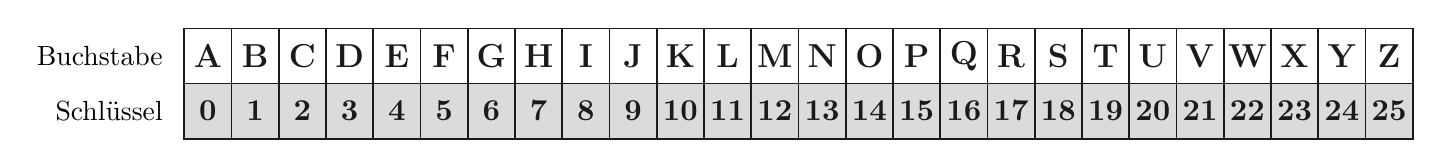
\begin{tikzpicture}
\node[font=\fs{10}, anchor=east] at (-0.15,1.05) {Buchstabe};
\node[font=\fs{10}, anchor=east] at (-0.15,0.35) {Schlüssel};
\draw[ink, line width=0.6pt] (0.0,0.7) rectangle ++(0.6,0.7) node[midway, font=\bfseries\fs{13}] {A};
\draw[ink, fill=black!14, line width=0.6pt] (0.0,0) rectangle ++(0.6,0.7) node[midway, font=\bfseries\fs{11}] {0};
\draw[ink, line width=0.6pt] (0.6,0.7) rectangle ++(0.6,0.7) node[midway, font=\bfseries\fs{13}] {B};
\draw[ink, fill=black!14, line width=0.6pt] (0.6,0) rectangle ++(0.6,0.7) node[midway, font=\bfseries\fs{11}] {1};
\draw[ink, line width=0.6pt] (1.2,0.7) rectangle ++(0.6,0.7) node[midway, font=\bfseries\fs{13}] {C};
\draw[ink, fill=black!14, line width=0.6pt] (1.2,0) rectangle ++(0.6,0.7) node[midway, font=\bfseries\fs{11}] {2};
\draw[ink, line width=0.6pt] (1.7999999999999998,0.7) rectangle ++(0.6,0.7) node[midway, font=\bfseries\fs{13}] {D};
\draw[ink, fill=black!14, line width=0.6pt] (1.7999999999999998,0) rectangle ++(0.6,0.7) node[midway, font=\bfseries\fs{11}] {3};
\draw[ink, line width=0.6pt] (2.4,0.7) rectangle ++(0.6,0.7) node[midway, font=\bfseries\fs{13}] {E};
\draw[ink, fill=black!14, line width=0.6pt] (2.4,0) rectangle ++(0.6,0.7) node[midway, font=\bfseries\fs{11}] {4};
\draw[ink, line width=0.6pt] (3.0,0.7) rectangle ++(0.6,0.7) node[midway, font=\bfseries\fs{13}] {F};
\draw[ink, fill=black!14, line width=0.6pt] (3.0,0) rectangle ++(0.6,0.7) node[midway, font=\bfseries\fs{11}] {5};
\draw[ink, line width=0.6pt] (3.5999999999999996,0.7) rectangle ++(0.6,0.7) node[midway, font=\bfseries\fs{13}] {G};
\draw[ink, fill=black!14, line width=0.6pt] (3.5999999999999996,0) rectangle ++(0.6,0.7) node[midway, font=\bfseries\fs{11}] {6};
\draw[ink, line width=0.6pt] (4.2,0.7) rectangle ++(0.6,0.7) node[midway, font=\bfseries\fs{13}] {H};
\draw[ink, fill=black!14, line width=0.6pt] (4.2,0) rectangle ++(0.6,0.7) node[midway, font=\bfseries\fs{11}] {7};
\draw[ink, line width=0.6pt] (4.8,0.7) rectangle ++(0.6,0.7) node[midway, font=\bfseries\fs{13}] {I};
\draw[ink, fill=black!14, line width=0.6pt] (4.8,0) rectangle ++(0.6,0.7) node[midway, font=\bfseries\fs{11}] {8};
\draw[ink, line width=0.6pt] (5.3999999999999995,0.7) rectangle ++(0.6,0.7) node[midway, font=\bfseries\fs{13}] {J};
\draw[ink, fill=black!14, line width=0.6pt] (5.3999999999999995,0) rectangle ++(0.6,0.7) node[midway, font=\bfseries\fs{11}] {9};
\draw[ink, line width=0.6pt] (6.0,0.7) rectangle ++(0.6,0.7) node[midway, font=\bfseries\fs{13}] {K};
\draw[ink, fill=black!14, line width=0.6pt] (6.0,0) rectangle ++(0.6,0.7) node[midway, font=\bfseries\fs{11}] {10};
\draw[ink, line width=0.6pt] (6.6,0.7) rectangle ++(0.6,0.7) node[midway, font=\bfseries\fs{13}] {L};
\draw[ink, fill=black!14, line width=0.6pt] (6.6,0) rectangle ++(0.6,0.7) node[midway, font=\bfseries\fs{11}] {11};
\draw[ink, line width=0.6pt] (7.199999999999999,0.7) rectangle ++(0.6,0.7) node[midway, font=\bfseries\fs{13}] {M};
\draw[ink, fill=black!14, line width=0.6pt] (7.199999999999999,0) rectangle ++(0.6,0.7) node[midway, font=\bfseries\fs{11}] {12};
\draw[ink, line width=0.6pt] (7.8,0.7) rectangle ++(0.6,0.7) node[midway, font=\bfseries\fs{13}] {N};
\draw[ink, fill=black!14, line width=0.6pt] (7.8,0) rectangle ++(0.6,0.7) node[midway, font=\bfseries\fs{11}] {13};
\draw[ink, line width=0.6pt] (8.4,0.7) rectangle ++(0.6,0.7) node[midway, font=\bfseries\fs{13}] {O};
\draw[ink, fill=black!14, line width=0.6pt] (8.4,0) rectangle ++(0.6,0.7) node[midway, font=\bfseries\fs{11}] {14};
\draw[ink, line width=0.6pt] (9.0,0.7) rectangle ++(0.6,0.7) node[midway, font=\bfseries\fs{13}] {P};
\draw[ink, fill=black!14, line width=0.6pt] (9.0,0) rectangle ++(0.6,0.7) node[midway, font=\bfseries\fs{11}] {15};
\draw[ink, line width=0.6pt] (9.6,0.7) rectangle ++(0.6,0.7) node[midway, font=\bfseries\fs{13}] {Q};
\draw[ink, fill=black!14, line width=0.6pt] (9.6,0) rectangle ++(0.6,0.7) node[midway, font=\bfseries\fs{11}] {16};
\draw[ink, line width=0.6pt] (10.2,0.7) rectangle ++(0.6,0.7) node[midway, font=\bfseries\fs{13}] {R};
\draw[ink, fill=black!14, line width=0.6pt] (10.2,0) rectangle ++(0.6,0.7) node[midway, font=\bfseries\fs{11}] {17};
\draw[ink, line width=0.6pt] (10.799999999999999,0.7) rectangle ++(0.6,0.7) node[midway, font=\bfseries\fs{13}] {S};
\draw[ink, fill=black!14, line width=0.6pt] (10.799999999999999,0) rectangle ++(0.6,0.7) node[midway, font=\bfseries\fs{11}] {18};
\draw[ink, line width=0.6pt] (11.4,0.7) rectangle ++(0.6,0.7) node[midway, font=\bfseries\fs{13}] {T};
\draw[ink, fill=black!14, line width=0.6pt] (11.4,0) rectangle ++(0.6,0.7) node[midway, font=\bfseries\fs{11}] {19};
\draw[ink, line width=0.6pt] (12.0,0.7) rectangle ++(0.6,0.7) node[midway, font=\bfseries\fs{13}] {U};
\draw[ink, fill=black!14, line width=0.6pt] (12.0,0) rectangle ++(0.6,0.7) node[midway, font=\bfseries\fs{11}] {20};
\draw[ink, line width=0.6pt] (12.6,0.7) rectangle ++(0.6,0.7) node[midway, font=\bfseries\fs{13}] {V};
\draw[ink, fill=black!14, line width=0.6pt] (12.6,0) rectangle ++(0.6,0.7) node[midway, font=\bfseries\fs{11}] {21};
\draw[ink, line width=0.6pt] (13.2,0.7) rectangle ++(0.6,0.7) node[midway, font=\bfseries\fs{13}] {W};
\draw[ink, fill=black!14, line width=0.6pt] (13.2,0) rectangle ++(0.6,0.7) node[midway, font=\bfseries\fs{11}] {22};
\draw[ink, line width=0.6pt] (13.799999999999999,0.7) rectangle ++(0.6,0.7) node[midway, font=\bfseries\fs{13}] {X};
\draw[ink, fill=black!14, line width=0.6pt] (13.799999999999999,0) rectangle ++(0.6,0.7) node[midway, font=\bfseries\fs{11}] {23};
\draw[ink, line width=0.6pt] (14.399999999999999,0.7) rectangle ++(0.6,0.7) node[midway, font=\bfseries\fs{13}] {Y};
\draw[ink, fill=black!14, line width=0.6pt] (14.399999999999999,0) rectangle ++(0.6,0.7) node[midway, font=\bfseries\fs{11}] {24};
\draw[ink, line width=0.6pt] (15.0,0.7) rectangle ++(0.6,0.7) node[midway, font=\bfseries\fs{13}] {Z};
\draw[ink, fill=black!14, line width=0.6pt] (15.0,0) rectangle ++(0.6,0.7) node[midway, font=\bfseries\fs{11}] {25};
\end{tikzpicture}\par\vspace{2.5mm}
{\fs{11} Das Codewort ist \textbf{FEE}, also die Schlüssel 5, 4, 4 – und dann wieder von vorn. Was steht hier?}\par\vspace{1.5mm}
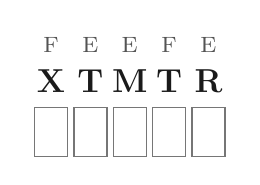
\begin{tikzpicture}
\node[font=\mono\bfseries\fs{13}, text=ink] at (0.25,0.95) {X};
\draw[ink!60, line width=0.5pt] (0.04,0) rectangle (0.46,0.62);
\node[font=\fs{8.5}, text=ink!75] at (0.25,1.42) {F};
\node[font=\mono\bfseries\fs{13}, text=ink] at (0.75,0.95) {T};
\draw[ink!60, line width=0.5pt] (0.54,0) rectangle (0.96,0.62);
\node[font=\fs{8.5}, text=ink!75] at (0.75,1.42) {E};
\node[font=\mono\bfseries\fs{13}, text=ink] at (1.25,0.95) {M};
\draw[ink!60, line width=0.5pt] (1.04,0) rectangle (1.46,0.62);
\node[font=\fs{8.5}, text=ink!75] at (1.25,1.42) {E};
\node[font=\mono\bfseries\fs{13}, text=ink] at (1.75,0.95) {T};
\draw[ink!60, line width=0.5pt] (1.54,0) rectangle (1.96,0.62);
\node[font=\fs{8.5}, text=ink!75] at (1.75,1.42) {F};
\node[font=\mono\bfseries\fs{13}, text=ink] at (2.25,0.95) {R};
\draw[ink!60, line width=0.5pt] (2.04,0) rectangle (2.46,0.62);
\node[font=\fs{8.5}, text=ink!75] at (2.25,1.42) {E};
\end{tikzpicture}\par
\vspace{3.5mm}

{\display\color{klar}\bfseries\fs{12} Was Codeknacker wissen}\par\vspace{1.5mm}
{\fs{10.5}
\textbf{Trick 1:} Alle Schlüssel ausprobieren. Bei einer einfachen Verschiebung gibt es nur 25.\par\vspace{1mm}
\textbf{Trick 2:} Buchstaben zählen. Der häufigste ist meistens das verkleidete E.\par\vspace{1mm}
\textbf{Bei einem Codewort:} In Teams zählen – so viele Teams, wie das Codewort Buchstaben hat.\par}
\vspace{3.5mm}

\aufgabe{Für Codeknacker: die Geheimbotschaft des Tages}{}
{\fs{11} \textbf{Erster Teil} – einfache Verschiebung, Schlüssel unbekannt:}\par\vspace{1.5mm}

\begin{tikzpicture}
\draw[wandblau, line width=2.2pt, rounded corners=6pt] (-0.3,-0.25) rectangle (16.3,1.4);
\node[font=\mono\bfseries\fs{13}, text=ink] at (0.25,0.95) {H};
\draw[ink!60, line width=0.5pt] (0.04,0) rectangle (0.46,0.62);
\node[font=\mono\bfseries\fs{13}, text=ink] at (0.75,0.95) {I};
\draw[ink!60, line width=0.5pt] (0.54,0) rectangle (0.96,0.62);
\node[font=\mono\bfseries\fs{13}, text=ink] at (1.25,0.95) {V};
\draw[ink!60, line width=0.5pt] (1.04,0) rectangle (1.46,0.62);
\node[font=\mono\bfseries\fs{13}, text=ink] at (2.25,0.95) {W};
\draw[ink!60, line width=0.5pt] (2.04,0) rectangle (2.46,0.62);
\node[font=\mono\bfseries\fs{13}, text=ink] at (2.75,0.95) {G};
\draw[ink!60, line width=0.5pt] (2.54,0) rectangle (2.96,0.62);
\node[font=\mono\bfseries\fs{13}, text=ink] at (3.25,0.95) {L};
\draw[ink!60, line width=0.5pt] (3.04,0) rectangle (3.46,0.62);
\node[font=\mono\bfseries\fs{13}, text=ink] at (3.75,0.95) {P};
\draw[ink!60, line width=0.5pt] (3.54,0) rectangle (3.96,0.62);
\node[font=\mono\bfseries\fs{13}, text=ink] at (4.25,0.95) {Y};
\draw[ink!60, line width=0.5pt] (4.04,0) rectangle (4.46,0.62);
\node[font=\mono\bfseries\fs{13}, text=ink] at (4.75,0.95) {I};
\draw[ink!60, line width=0.5pt] (4.54,0) rectangle (4.96,0.62);
\node[font=\mono\bfseries\fs{13}, text=ink] at (5.25,0.95) {W};
\draw[ink!60, line width=0.5pt] (5.04,0) rectangle (5.46,0.62);
\node[font=\mono\bfseries\fs{13}, text=ink] at (5.75,0.95) {W};
\draw[ink!60, line width=0.5pt] (5.54,0) rectangle (5.96,0.62);
\node[font=\mono\bfseries\fs{13}, text=ink] at (6.25,0.95) {I};
\draw[ink!60, line width=0.5pt] (6.04,0) rectangle (6.46,0.62);
\node[font=\mono\bfseries\fs{13}, text=ink] at (6.75,0.95) {P};
\draw[ink!60, line width=0.5pt] (6.54,0) rectangle (6.96,0.62);
\node[font=\mono\bfseries\fs{13}, text=ink] at (7.75,0.95) {M};
\draw[ink!60, line width=0.5pt] (7.54,0) rectangle (7.96,0.62);
\node[font=\mono\bfseries\fs{13}, text=ink] at (8.25,0.95) {W};
\draw[ink!60, line width=0.5pt] (8.04,0) rectangle (8.46,0.62);
\node[font=\mono\bfseries\fs{13}, text=ink] at (8.75,0.95) {X};
\draw[ink!60, line width=0.5pt] (8.54,0) rectangle (8.96,0.62);
\node[font=\mono\bfseries\fs{13}, text=ink] at (9.75,0.95) {H};
\draw[ink!60, line width=0.5pt] (9.54,0) rectangle (9.96,0.62);
\node[font=\mono\bfseries\fs{13}, text=ink] at (10.25,0.95) {V};
\draw[ink!60, line width=0.5pt] (10.04,0) rectangle (10.46,0.62);
\node[font=\mono\bfseries\fs{13}, text=ink] at (10.75,0.95) {I};
\draw[ink!60, line width=0.5pt] (10.54,0) rectangle (10.96,0.62);
\node[font=\mono\bfseries\fs{13}, text=ink] at (11.25,0.95) {M};
\draw[ink!60, line width=0.5pt] (11.04,0) rectangle (11.46,0.62);
\node[font=\mono\bfseries\fs{13}, text=ink] at (12.25,0.95) {Y};
\draw[ink!60, line width=0.5pt] (12.04,0) rectangle (12.46,0.62);
\node[font=\mono\bfseries\fs{13}, text=ink] at (12.75,0.95) {R};
\draw[ink!60, line width=0.5pt] (12.54,0) rectangle (12.96,0.62);
\node[font=\mono\bfseries\fs{13}, text=ink] at (13.25,0.95) {H};
\draw[ink!60, line width=0.5pt] (13.04,0) rectangle (13.46,0.62);
\node[font=\mono\bfseries\fs{13}, text=ink] at (14.25,0.95) {I};
\draw[ink!60, line width=0.5pt] (14.04,0) rectangle (14.46,0.62);
\node[font=\mono\bfseries\fs{13}, text=ink] at (14.75,0.95) {M};
\draw[ink!60, line width=0.5pt] (14.54,0) rectangle (14.96,0.62);
\node[font=\mono\bfseries\fs{13}, text=ink] at (15.25,0.95) {R};
\draw[ink!60, line width=0.5pt] (15.04,0) rectangle (15.46,0.62);
\node[font=\mono\bfseries\fs{13}, text=ink] at (15.75,0.95) {W};
\draw[ink!60, line width=0.5pt] (15.54,0) rectangle (15.96,0.62);
\end{tikzpicture}\par\vspace{3mm}
{\fs{11} \textbf{Zweiter Teil} – die Schlüssel verrät dir der erste Teil:}\par\vspace{1.5mm}
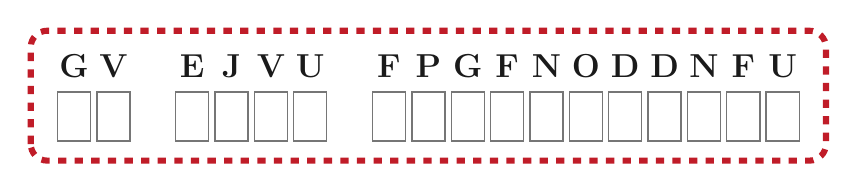
\begin{tikzpicture}
\draw[wandrot, dashed, line width=2.2pt, rounded corners=6pt] (-0.3,-0.25) rectangle (9.8,1.4);
\node[font=\mono\bfseries\fs{13}, text=ink] at (0.25,0.95) {G};
\draw[ink!60, line width=0.5pt] (0.04,0) rectangle (0.46,0.62);
\node[font=\mono\bfseries\fs{13}, text=ink] at (0.75,0.95) {V};
\draw[ink!60, line width=0.5pt] (0.54,0) rectangle (0.96,0.62);
\node[font=\mono\bfseries\fs{13}, text=ink] at (1.75,0.95) {E};
\draw[ink!60, line width=0.5pt] (1.54,0) rectangle (1.96,0.62);
\node[font=\mono\bfseries\fs{13}, text=ink] at (2.25,0.95) {J};
\draw[ink!60, line width=0.5pt] (2.04,0) rectangle (2.46,0.62);
\node[font=\mono\bfseries\fs{13}, text=ink] at (2.75,0.95) {V};
\draw[ink!60, line width=0.5pt] (2.54,0) rectangle (2.96,0.62);
\node[font=\mono\bfseries\fs{13}, text=ink] at (3.25,0.95) {U};
\draw[ink!60, line width=0.5pt] (3.04,0) rectangle (3.46,0.62);
\node[font=\mono\bfseries\fs{13}, text=ink] at (4.25,0.95) {F};
\draw[ink!60, line width=0.5pt] (4.04,0) rectangle (4.46,0.62);
\node[font=\mono\bfseries\fs{13}, text=ink] at (4.75,0.95) {P};
\draw[ink!60, line width=0.5pt] (4.54,0) rectangle (4.96,0.62);
\node[font=\mono\bfseries\fs{13}, text=ink] at (5.25,0.95) {G};
\draw[ink!60, line width=0.5pt] (5.04,0) rectangle (5.46,0.62);
\node[font=\mono\bfseries\fs{13}, text=ink] at (5.75,0.95) {F};
\draw[ink!60, line width=0.5pt] (5.54,0) rectangle (5.96,0.62);
\node[font=\mono\bfseries\fs{13}, text=ink] at (6.25,0.95) {N};
\draw[ink!60, line width=0.5pt] (6.04,0) rectangle (6.46,0.62);
\node[font=\mono\bfseries\fs{13}, text=ink] at (6.75,0.95) {O};
\draw[ink!60, line width=0.5pt] (6.54,0) rectangle (6.96,0.62);
\node[font=\mono\bfseries\fs{13}, text=ink] at (7.25,0.95) {D};
\draw[ink!60, line width=0.5pt] (7.04,0) rectangle (7.46,0.62);
\node[font=\mono\bfseries\fs{13}, text=ink] at (7.75,0.95) {D};
\draw[ink!60, line width=0.5pt] (7.54,0) rectangle (7.96,0.62);
\node[font=\mono\bfseries\fs{13}, text=ink] at (8.25,0.95) {N};
\draw[ink!60, line width=0.5pt] (8.04,0) rectangle (8.46,0.62);
\node[font=\mono\bfseries\fs{13}, text=ink] at (8.75,0.95) {F};
\draw[ink!60, line width=0.5pt] (8.54,0) rectangle (8.96,0.62);
\node[font=\mono\bfseries\fs{13}, text=ink] at (9.25,0.95) {U};
\draw[ink!60, line width=0.5pt] (9.04,0) rectangle (9.46,0.62);
\end{tikzpicture}\par

\newpage
{\display\fs{28}\color{klar} RÄTSEL FÜR ZU HAUSE}\hfill{\fs{10.5} Kinder-Uni der RPTU · Prof. Dr. Max Horn}\par
\vspace{2mm}
{\fs{10.5} Tipp: Nimm die Caesar-Scheibe oder den Buchstabenkreis. Lösungen stehen unten, kopfüber.}\par
\vspace{5mm}

\aufgabe{1 · Zum Aufwärmen}{Schlüssel 3}
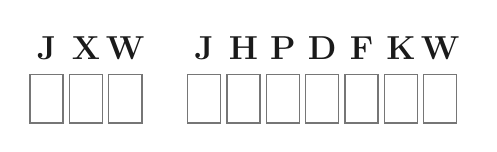
\begin{tikzpicture}
\node[font=\mono\bfseries\fs{13}, text=ink] at (0.25,0.95) {J};
\draw[ink!60, line width=0.5pt] (0.04,0) rectangle (0.46,0.62);
\node[font=\mono\bfseries\fs{13}, text=ink] at (0.75,0.95) {X};
\draw[ink!60, line width=0.5pt] (0.54,0) rectangle (0.96,0.62);
\node[font=\mono\bfseries\fs{13}, text=ink] at (1.25,0.95) {W};
\draw[ink!60, line width=0.5pt] (1.04,0) rectangle (1.46,0.62);
\node[font=\mono\bfseries\fs{13}, text=ink] at (2.25,0.95) {J};
\draw[ink!60, line width=0.5pt] (2.04,0) rectangle (2.46,0.62);
\node[font=\mono\bfseries\fs{13}, text=ink] at (2.75,0.95) {H};
\draw[ink!60, line width=0.5pt] (2.54,0) rectangle (2.96,0.62);
\node[font=\mono\bfseries\fs{13}, text=ink] at (3.25,0.95) {P};
\draw[ink!60, line width=0.5pt] (3.04,0) rectangle (3.46,0.62);
\node[font=\mono\bfseries\fs{13}, text=ink] at (3.75,0.95) {D};
\draw[ink!60, line width=0.5pt] (3.54,0) rectangle (3.96,0.62);
\node[font=\mono\bfseries\fs{13}, text=ink] at (4.25,0.95) {F};
\draw[ink!60, line width=0.5pt] (4.04,0) rectangle (4.46,0.62);
\node[font=\mono\bfseries\fs{13}, text=ink] at (4.75,0.95) {K};
\draw[ink!60, line width=0.5pt] (4.54,0) rectangle (4.96,0.62);
\node[font=\mono\bfseries\fs{13}, text=ink] at (5.25,0.95) {W};
\draw[ink!60, line width=0.5pt] (5.04,0) rectangle (5.46,0.62);
\end{tikzpicture}\par\vspace{5mm}

\aufgabe{2 · Schon schwerer}{Schlüssel 10}

\begin{tikzpicture}
\node[font=\mono\bfseries\fs{13}, text=ink] at (0.25,0.95) {W};
\draw[ink!60, line width=0.5pt] (0.04,0) rectangle (0.46,0.62);
\node[font=\mono\bfseries\fs{13}, text=ink] at (0.75,0.95) {K};
\draw[ink!60, line width=0.5pt] (0.54,0) rectangle (0.96,0.62);
\node[font=\mono\bfseries\fs{13}, text=ink] at (1.25,0.95) {D};
\draw[ink!60, line width=0.5pt] (1.04,0) rectangle (1.46,0.62);
\node[font=\mono\bfseries\fs{13}, text=ink] at (1.75,0.95) {R};
\draw[ink!60, line width=0.5pt] (1.54,0) rectangle (1.96,0.62);
\node[font=\mono\bfseries\fs{13}, text=ink] at (2.25,0.95) {O};
\draw[ink!60, line width=0.5pt] (2.04,0) rectangle (2.46,0.62);
\node[font=\mono\bfseries\fs{13}, text=ink] at (3.25,0.95) {W};
\draw[ink!60, line width=0.5pt] (3.04,0) rectangle (3.46,0.62);
\node[font=\mono\bfseries\fs{13}, text=ink] at (3.75,0.95) {K};
\draw[ink!60, line width=0.5pt] (3.54,0) rectangle (3.96,0.62);
\node[font=\mono\bfseries\fs{13}, text=ink] at (4.25,0.95) {M};
\draw[ink!60, line width=0.5pt] (4.04,0) rectangle (4.46,0.62);
\node[font=\mono\bfseries\fs{13}, text=ink] at (4.75,0.95) {R};
\draw[ink!60, line width=0.5pt] (4.54,0) rectangle (4.96,0.62);
\node[font=\mono\bfseries\fs{13}, text=ink] at (5.25,0.95) {D};
\draw[ink!60, line width=0.5pt] (5.04,0) rectangle (5.46,0.62);
\node[font=\mono\bfseries\fs{13}, text=ink] at (6.25,0.95) {C};
\draw[ink!60, line width=0.5pt] (6.04,0) rectangle (6.46,0.62);
\node[font=\mono\bfseries\fs{13}, text=ink] at (6.75,0.95) {Z};
\draw[ink!60, line width=0.5pt] (6.54,0) rectangle (6.96,0.62);
\node[font=\mono\bfseries\fs{13}, text=ink] at (7.25,0.95) {K};
\draw[ink!60, line width=0.5pt] (7.04,0) rectangle (7.46,0.62);
\node[font=\mono\bfseries\fs{13}, text=ink] at (7.75,0.95) {C};
\draw[ink!60, line width=0.5pt] (7.54,0) rectangle (7.96,0.62);
\node[font=\mono\bfseries\fs{13}, text=ink] at (8.25,0.95) {C};
\draw[ink!60, line width=0.5pt] (8.04,0) rectangle (8.46,0.62);
\end{tikzpicture}\par\vspace{5mm}

\aufgabe{3 · Für Codeknacker}{Schlüssel unbekannt! Zähle: Welcher Buchstabe ist das verkleidete E?}
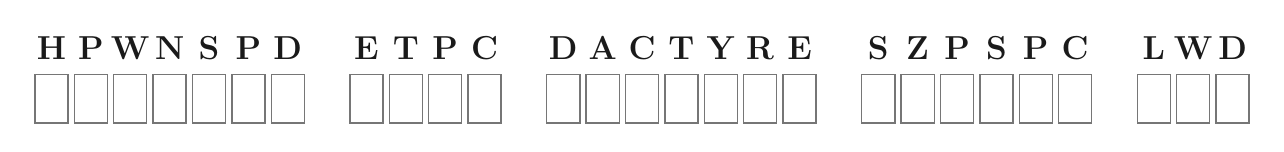
\begin{tikzpicture}
\node[font=\mono\bfseries\fs{13}, text=ink] at (0.25,0.95) {H};
\draw[ink!60, line width=0.5pt] (0.04,0) rectangle (0.46,0.62);
\node[font=\mono\bfseries\fs{13}, text=ink] at (0.75,0.95) {P};
\draw[ink!60, line width=0.5pt] (0.54,0) rectangle (0.96,0.62);
\node[font=\mono\bfseries\fs{13}, text=ink] at (1.25,0.95) {W};
\draw[ink!60, line width=0.5pt] (1.04,0) rectangle (1.46,0.62);
\node[font=\mono\bfseries\fs{13}, text=ink] at (1.75,0.95) {N};
\draw[ink!60, line width=0.5pt] (1.54,0) rectangle (1.96,0.62);
\node[font=\mono\bfseries\fs{13}, text=ink] at (2.25,0.95) {S};
\draw[ink!60, line width=0.5pt] (2.04,0) rectangle (2.46,0.62);
\node[font=\mono\bfseries\fs{13}, text=ink] at (2.75,0.95) {P};
\draw[ink!60, line width=0.5pt] (2.54,0) rectangle (2.96,0.62);
\node[font=\mono\bfseries\fs{13}, text=ink] at (3.25,0.95) {D};
\draw[ink!60, line width=0.5pt] (3.04,0) rectangle (3.46,0.62);
\node[font=\mono\bfseries\fs{13}, text=ink] at (4.25,0.95) {E};
\draw[ink!60, line width=0.5pt] (4.04,0) rectangle (4.46,0.62);
\node[font=\mono\bfseries\fs{13}, text=ink] at (4.75,0.95) {T};
\draw[ink!60, line width=0.5pt] (4.54,0) rectangle (4.96,0.62);
\node[font=\mono\bfseries\fs{13}, text=ink] at (5.25,0.95) {P};
\draw[ink!60, line width=0.5pt] (5.04,0) rectangle (5.46,0.62);
\node[font=\mono\bfseries\fs{13}, text=ink] at (5.75,0.95) {C};
\draw[ink!60, line width=0.5pt] (5.54,0) rectangle (5.96,0.62);
\node[font=\mono\bfseries\fs{13}, text=ink] at (6.75,0.95) {D};
\draw[ink!60, line width=0.5pt] (6.54,0) rectangle (6.96,0.62);
\node[font=\mono\bfseries\fs{13}, text=ink] at (7.25,0.95) {A};
\draw[ink!60, line width=0.5pt] (7.04,0) rectangle (7.46,0.62);
\node[font=\mono\bfseries\fs{13}, text=ink] at (7.75,0.95) {C};
\draw[ink!60, line width=0.5pt] (7.54,0) rectangle (7.96,0.62);
\node[font=\mono\bfseries\fs{13}, text=ink] at (8.25,0.95) {T};
\draw[ink!60, line width=0.5pt] (8.04,0) rectangle (8.46,0.62);
\node[font=\mono\bfseries\fs{13}, text=ink] at (8.75,0.95) {Y};
\draw[ink!60, line width=0.5pt] (8.54,0) rectangle (8.96,0.62);
\node[font=\mono\bfseries\fs{13}, text=ink] at (9.25,0.95) {R};
\draw[ink!60, line width=0.5pt] (9.04,0) rectangle (9.46,0.62);
\node[font=\mono\bfseries\fs{13}, text=ink] at (9.75,0.95) {E};
\draw[ink!60, line width=0.5pt] (9.54,0) rectangle (9.96,0.62);
\node[font=\mono\bfseries\fs{13}, text=ink] at (10.75,0.95) {S};
\draw[ink!60, line width=0.5pt] (10.54,0) rectangle (10.96,0.62);
\node[font=\mono\bfseries\fs{13}, text=ink] at (11.25,0.95) {Z};
\draw[ink!60, line width=0.5pt] (11.04,0) rectangle (11.46,0.62);
\node[font=\mono\bfseries\fs{13}, text=ink] at (11.75,0.95) {P};
\draw[ink!60, line width=0.5pt] (11.54,0) rectangle (11.96,0.62);
\node[font=\mono\bfseries\fs{13}, text=ink] at (12.25,0.95) {S};
\draw[ink!60, line width=0.5pt] (12.04,0) rectangle (12.46,0.62);
\node[font=\mono\bfseries\fs{13}, text=ink] at (12.75,0.95) {P};
\draw[ink!60, line width=0.5pt] (12.54,0) rectangle (12.96,0.62);
\node[font=\mono\bfseries\fs{13}, text=ink] at (13.25,0.95) {C};
\draw[ink!60, line width=0.5pt] (13.04,0) rectangle (13.46,0.62);
\node[font=\mono\bfseries\fs{13}, text=ink] at (14.25,0.95) {L};
\draw[ink!60, line width=0.5pt] (14.04,0) rectangle (14.46,0.62);
\node[font=\mono\bfseries\fs{13}, text=ink] at (14.75,0.95) {W};
\draw[ink!60, line width=0.5pt] (14.54,0) rectangle (14.96,0.62);
\node[font=\mono\bfseries\fs{13}, text=ink] at (15.25,0.95) {D};
\draw[ink!60, line width=0.5pt] (15.04,0) rectangle (15.46,0.62);
\end{tikzpicture}

\vspace{1.5mm}
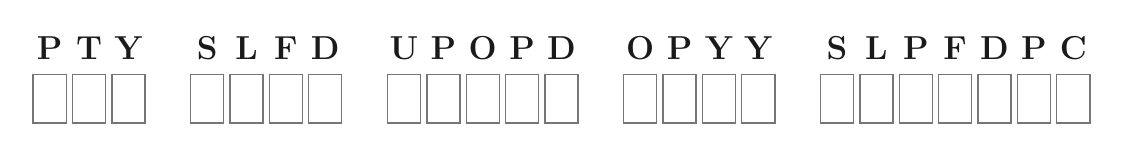
\begin{tikzpicture}
\node[font=\mono\bfseries\fs{13}, text=ink] at (0.25,0.95) {P};
\draw[ink!60, line width=0.5pt] (0.04,0) rectangle (0.46,0.62);
\node[font=\mono\bfseries\fs{13}, text=ink] at (0.75,0.95) {T};
\draw[ink!60, line width=0.5pt] (0.54,0) rectangle (0.96,0.62);
\node[font=\mono\bfseries\fs{13}, text=ink] at (1.25,0.95) {Y};
\draw[ink!60, line width=0.5pt] (1.04,0) rectangle (1.46,0.62);
\node[font=\mono\bfseries\fs{13}, text=ink] at (2.25,0.95) {S};
\draw[ink!60, line width=0.5pt] (2.04,0) rectangle (2.46,0.62);
\node[font=\mono\bfseries\fs{13}, text=ink] at (2.75,0.95) {L};
\draw[ink!60, line width=0.5pt] (2.54,0) rectangle (2.96,0.62);
\node[font=\mono\bfseries\fs{13}, text=ink] at (3.25,0.95) {F};
\draw[ink!60, line width=0.5pt] (3.04,0) rectangle (3.46,0.62);
\node[font=\mono\bfseries\fs{13}, text=ink] at (3.75,0.95) {D};
\draw[ink!60, line width=0.5pt] (3.54,0) rectangle (3.96,0.62);
\node[font=\mono\bfseries\fs{13}, text=ink] at (4.75,0.95) {U};
\draw[ink!60, line width=0.5pt] (4.54,0) rectangle (4.96,0.62);
\node[font=\mono\bfseries\fs{13}, text=ink] at (5.25,0.95) {P};
\draw[ink!60, line width=0.5pt] (5.04,0) rectangle (5.46,0.62);
\node[font=\mono\bfseries\fs{13}, text=ink] at (5.75,0.95) {O};
\draw[ink!60, line width=0.5pt] (5.54,0) rectangle (5.96,0.62);
\node[font=\mono\bfseries\fs{13}, text=ink] at (6.25,0.95) {P};
\draw[ink!60, line width=0.5pt] (6.04,0) rectangle (6.46,0.62);
\node[font=\mono\bfseries\fs{13}, text=ink] at (6.75,0.95) {D};
\draw[ink!60, line width=0.5pt] (6.54,0) rectangle (6.96,0.62);
\node[font=\mono\bfseries\fs{13}, text=ink] at (7.75,0.95) {O};
\draw[ink!60, line width=0.5pt] (7.54,0) rectangle (7.96,0.62);
\node[font=\mono\bfseries\fs{13}, text=ink] at (8.25,0.95) {P};
\draw[ink!60, line width=0.5pt] (8.04,0) rectangle (8.46,0.62);
\node[font=\mono\bfseries\fs{13}, text=ink] at (8.75,0.95) {Y};
\draw[ink!60, line width=0.5pt] (8.54,0) rectangle (8.96,0.62);
\node[font=\mono\bfseries\fs{13}, text=ink] at (9.25,0.95) {Y};
\draw[ink!60, line width=0.5pt] (9.04,0) rectangle (9.46,0.62);
\node[font=\mono\bfseries\fs{13}, text=ink] at (10.25,0.95) {S};
\draw[ink!60, line width=0.5pt] (10.04,0) rectangle (10.46,0.62);
\node[font=\mono\bfseries\fs{13}, text=ink] at (10.75,0.95) {L};
\draw[ink!60, line width=0.5pt] (10.54,0) rectangle (10.96,0.62);
\node[font=\mono\bfseries\fs{13}, text=ink] at (11.25,0.95) {P};
\draw[ink!60, line width=0.5pt] (11.04,0) rectangle (11.46,0.62);
\node[font=\mono\bfseries\fs{13}, text=ink] at (11.75,0.95) {F};
\draw[ink!60, line width=0.5pt] (11.54,0) rectangle (11.96,0.62);
\node[font=\mono\bfseries\fs{13}, text=ink] at (12.25,0.95) {D};
\draw[ink!60, line width=0.5pt] (12.04,0) rectangle (12.46,0.62);
\node[font=\mono\bfseries\fs{13}, text=ink] at (12.75,0.95) {P};
\draw[ink!60, line width=0.5pt] (12.54,0) rectangle (12.96,0.62);
\node[font=\mono\bfseries\fs{13}, text=ink] at (13.25,0.95) {C};
\draw[ink!60, line width=0.5pt] (13.04,0) rectangle (13.46,0.62);
\end{tikzpicture}

\vspace{1.5mm}
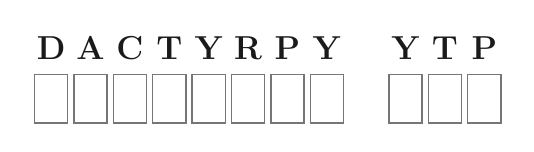
\begin{tikzpicture}
\node[font=\mono\bfseries\fs{13}, text=ink] at (0.25,0.95) {D};
\draw[ink!60, line width=0.5pt] (0.04,0) rectangle (0.46,0.62);
\node[font=\mono\bfseries\fs{13}, text=ink] at (0.75,0.95) {A};
\draw[ink!60, line width=0.5pt] (0.54,0) rectangle (0.96,0.62);
\node[font=\mono\bfseries\fs{13}, text=ink] at (1.25,0.95) {C};
\draw[ink!60, line width=0.5pt] (1.04,0) rectangle (1.46,0.62);
\node[font=\mono\bfseries\fs{13}, text=ink] at (1.75,0.95) {T};
\draw[ink!60, line width=0.5pt] (1.54,0) rectangle (1.96,0.62);
\node[font=\mono\bfseries\fs{13}, text=ink] at (2.25,0.95) {Y};
\draw[ink!60, line width=0.5pt] (2.04,0) rectangle (2.46,0.62);
\node[font=\mono\bfseries\fs{13}, text=ink] at (2.75,0.95) {R};
\draw[ink!60, line width=0.5pt] (2.54,0) rectangle (2.96,0.62);
\node[font=\mono\bfseries\fs{13}, text=ink] at (3.25,0.95) {P};
\draw[ink!60, line width=0.5pt] (3.04,0) rectangle (3.46,0.62);
\node[font=\mono\bfseries\fs{13}, text=ink] at (3.75,0.95) {Y};
\draw[ink!60, line width=0.5pt] (3.54,0) rectangle (3.96,0.62);
\node[font=\mono\bfseries\fs{13}, text=ink] at (4.75,0.95) {Y};
\draw[ink!60, line width=0.5pt] (4.54,0) rectangle (4.96,0.62);
\node[font=\mono\bfseries\fs{13}, text=ink] at (5.25,0.95) {T};
\draw[ink!60, line width=0.5pt] (5.04,0) rectangle (5.46,0.62);
\node[font=\mono\bfseries\fs{13}, text=ink] at (5.75,0.95) {P};
\draw[ink!60, line width=0.5pt] (5.54,0) rectangle (5.96,0.62);
\end{tikzpicture}\par\vspace{5mm}

\aufgabe{4 · Für Profis}{Das Codewort ist FCK. Die Zahlentabelle steht auf der Vorderseite.}
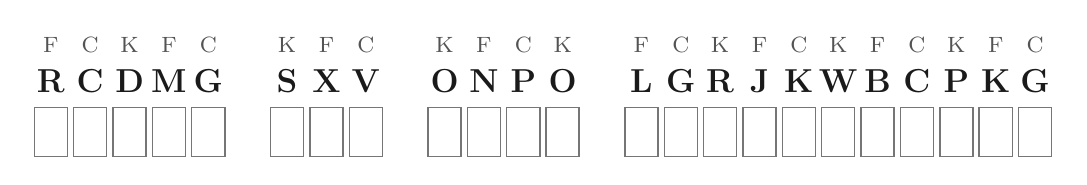
\begin{tikzpicture}
\node[font=\mono\bfseries\fs{13}, text=ink] at (0.25,0.95) {R};
\draw[ink!60, line width=0.5pt] (0.04,0) rectangle (0.46,0.62);
\node[font=\fs{8.5}, text=ink!75] at (0.25,1.42) {F};
\node[font=\mono\bfseries\fs{13}, text=ink] at (0.75,0.95) {C};
\draw[ink!60, line width=0.5pt] (0.54,0) rectangle (0.96,0.62);
\node[font=\fs{8.5}, text=ink!75] at (0.75,1.42) {C};
\node[font=\mono\bfseries\fs{13}, text=ink] at (1.25,0.95) {D};
\draw[ink!60, line width=0.5pt] (1.04,0) rectangle (1.46,0.62);
\node[font=\fs{8.5}, text=ink!75] at (1.25,1.42) {K};
\node[font=\mono\bfseries\fs{13}, text=ink] at (1.75,0.95) {M};
\draw[ink!60, line width=0.5pt] (1.54,0) rectangle (1.96,0.62);
\node[font=\fs{8.5}, text=ink!75] at (1.75,1.42) {F};
\node[font=\mono\bfseries\fs{13}, text=ink] at (2.25,0.95) {G};
\draw[ink!60, line width=0.5pt] (2.04,0) rectangle (2.46,0.62);
\node[font=\fs{8.5}, text=ink!75] at (2.25,1.42) {C};
\node[font=\mono\bfseries\fs{13}, text=ink] at (3.25,0.95) {S};
\draw[ink!60, line width=0.5pt] (3.04,0) rectangle (3.46,0.62);
\node[font=\fs{8.5}, text=ink!75] at (3.25,1.42) {K};
\node[font=\mono\bfseries\fs{13}, text=ink] at (3.75,0.95) {X};
\draw[ink!60, line width=0.5pt] (3.54,0) rectangle (3.96,0.62);
\node[font=\fs{8.5}, text=ink!75] at (3.75,1.42) {F};
\node[font=\mono\bfseries\fs{13}, text=ink] at (4.25,0.95) {V};
\draw[ink!60, line width=0.5pt] (4.04,0) rectangle (4.46,0.62);
\node[font=\fs{8.5}, text=ink!75] at (4.25,1.42) {C};
\node[font=\mono\bfseries\fs{13}, text=ink] at (5.25,0.95) {O};
\draw[ink!60, line width=0.5pt] (5.04,0) rectangle (5.46,0.62);
\node[font=\fs{8.5}, text=ink!75] at (5.25,1.42) {K};
\node[font=\mono\bfseries\fs{13}, text=ink] at (5.75,0.95) {N};
\draw[ink!60, line width=0.5pt] (5.54,0) rectangle (5.96,0.62);
\node[font=\fs{8.5}, text=ink!75] at (5.75,1.42) {F};
\node[font=\mono\bfseries\fs{13}, text=ink] at (6.25,0.95) {P};
\draw[ink!60, line width=0.5pt] (6.04,0) rectangle (6.46,0.62);
\node[font=\fs{8.5}, text=ink!75] at (6.25,1.42) {C};
\node[font=\mono\bfseries\fs{13}, text=ink] at (6.75,0.95) {O};
\draw[ink!60, line width=0.5pt] (6.54,0) rectangle (6.96,0.62);
\node[font=\fs{8.5}, text=ink!75] at (6.75,1.42) {K};
\node[font=\mono\bfseries\fs{13}, text=ink] at (7.75,0.95) {L};
\draw[ink!60, line width=0.5pt] (7.54,0) rectangle (7.96,0.62);
\node[font=\fs{8.5}, text=ink!75] at (7.75,1.42) {F};
\node[font=\mono\bfseries\fs{13}, text=ink] at (8.25,0.95) {G};
\draw[ink!60, line width=0.5pt] (8.04,0) rectangle (8.46,0.62);
\node[font=\fs{8.5}, text=ink!75] at (8.25,1.42) {C};
\node[font=\mono\bfseries\fs{13}, text=ink] at (8.75,0.95) {R};
\draw[ink!60, line width=0.5pt] (8.54,0) rectangle (8.96,0.62);
\node[font=\fs{8.5}, text=ink!75] at (8.75,1.42) {K};
\node[font=\mono\bfseries\fs{13}, text=ink] at (9.25,0.95) {J};
\draw[ink!60, line width=0.5pt] (9.04,0) rectangle (9.46,0.62);
\node[font=\fs{8.5}, text=ink!75] at (9.25,1.42) {F};
\node[font=\mono\bfseries\fs{13}, text=ink] at (9.75,0.95) {K};
\draw[ink!60, line width=0.5pt] (9.54,0) rectangle (9.96,0.62);
\node[font=\fs{8.5}, text=ink!75] at (9.75,1.42) {C};
\node[font=\mono\bfseries\fs{13}, text=ink] at (10.25,0.95) {W};
\draw[ink!60, line width=0.5pt] (10.04,0) rectangle (10.46,0.62);
\node[font=\fs{8.5}, text=ink!75] at (10.25,1.42) {K};
\node[font=\mono\bfseries\fs{13}, text=ink] at (10.75,0.95) {B};
\draw[ink!60, line width=0.5pt] (10.54,0) rectangle (10.96,0.62);
\node[font=\fs{8.5}, text=ink!75] at (10.75,1.42) {F};
\node[font=\mono\bfseries\fs{13}, text=ink] at (11.25,0.95) {C};
\draw[ink!60, line width=0.5pt] (11.04,0) rectangle (11.46,0.62);
\node[font=\fs{8.5}, text=ink!75] at (11.25,1.42) {C};
\node[font=\mono\bfseries\fs{13}, text=ink] at (11.75,0.95) {P};
\draw[ink!60, line width=0.5pt] (11.54,0) rectangle (11.96,0.62);
\node[font=\fs{8.5}, text=ink!75] at (11.75,1.42) {K};
\node[font=\mono\bfseries\fs{13}, text=ink] at (12.25,0.95) {K};
\draw[ink!60, line width=0.5pt] (12.04,0) rectangle (12.46,0.62);
\node[font=\fs{8.5}, text=ink!75] at (12.25,1.42) {F};
\node[font=\mono\bfseries\fs{13}, text=ink] at (12.75,0.95) {G};
\draw[ink!60, line width=0.5pt] (12.54,0) rectangle (12.96,0.62);
\node[font=\fs{8.5}, text=ink!75] at (12.75,1.42) {C};
\end{tikzpicture}\par\vspace{5mm}

\aufgabe{5 · Knobelfragen}{}
{\fs{11}
a) Was passiert, wenn du mit Schlüssel 26 verschlüsselst?\par\vspace{1.5mm}
b) Du verschlüsselst erst mit Schlüssel 3 und das Ergebnis noch einmal mit Schlüssel 5.
Welcher einzelne Schlüssel hätte dasselbe getan?\par\vspace{1.5mm}
c) Wie viele verschiedene Codewörter mit zwei Buchstaben gibt es?\par}
\vspace{5mm}

\aufgabe{6 · Deine eigene Geheimbotschaft}{Verschlüssle sie und verschenke sie.}
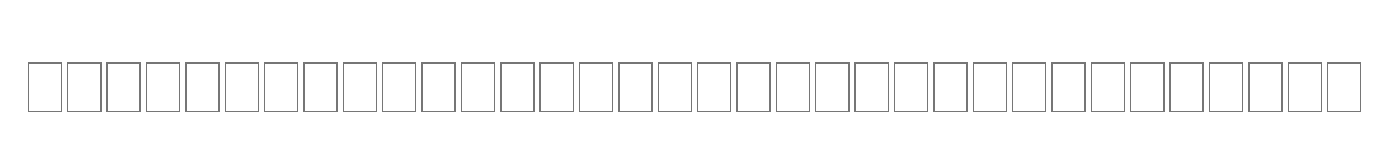
\begin{tikzpicture}
\node[font=\mono\bfseries\fs{13}, text=ink] at (0.25,0.95) {};
\draw[ink!60, line width=0.5pt] (0.04,0) rectangle (0.46,0.62);
\node[font=\mono\bfseries\fs{13}, text=ink] at (0.75,0.95) {};
\draw[ink!60, line width=0.5pt] (0.54,0) rectangle (0.96,0.62);
\node[font=\mono\bfseries\fs{13}, text=ink] at (1.25,0.95) {};
\draw[ink!60, line width=0.5pt] (1.04,0) rectangle (1.46,0.62);
\node[font=\mono\bfseries\fs{13}, text=ink] at (1.75,0.95) {};
\draw[ink!60, line width=0.5pt] (1.54,0) rectangle (1.96,0.62);
\node[font=\mono\bfseries\fs{13}, text=ink] at (2.25,0.95) {};
\draw[ink!60, line width=0.5pt] (2.04,0) rectangle (2.46,0.62);
\node[font=\mono\bfseries\fs{13}, text=ink] at (2.75,0.95) {};
\draw[ink!60, line width=0.5pt] (2.54,0) rectangle (2.96,0.62);
\node[font=\mono\bfseries\fs{13}, text=ink] at (3.25,0.95) {};
\draw[ink!60, line width=0.5pt] (3.04,0) rectangle (3.46,0.62);
\node[font=\mono\bfseries\fs{13}, text=ink] at (3.75,0.95) {};
\draw[ink!60, line width=0.5pt] (3.54,0) rectangle (3.96,0.62);
\node[font=\mono\bfseries\fs{13}, text=ink] at (4.25,0.95) {};
\draw[ink!60, line width=0.5pt] (4.04,0) rectangle (4.46,0.62);
\node[font=\mono\bfseries\fs{13}, text=ink] at (4.75,0.95) {};
\draw[ink!60, line width=0.5pt] (4.54,0) rectangle (4.96,0.62);
\node[font=\mono\bfseries\fs{13}, text=ink] at (5.25,0.95) {};
\draw[ink!60, line width=0.5pt] (5.04,0) rectangle (5.46,0.62);
\node[font=\mono\bfseries\fs{13}, text=ink] at (5.75,0.95) {};
\draw[ink!60, line width=0.5pt] (5.54,0) rectangle (5.96,0.62);
\node[font=\mono\bfseries\fs{13}, text=ink] at (6.25,0.95) {};
\draw[ink!60, line width=0.5pt] (6.04,0) rectangle (6.46,0.62);
\node[font=\mono\bfseries\fs{13}, text=ink] at (6.75,0.95) {};
\draw[ink!60, line width=0.5pt] (6.54,0) rectangle (6.96,0.62);
\node[font=\mono\bfseries\fs{13}, text=ink] at (7.25,0.95) {};
\draw[ink!60, line width=0.5pt] (7.04,0) rectangle (7.46,0.62);
\node[font=\mono\bfseries\fs{13}, text=ink] at (7.75,0.95) {};
\draw[ink!60, line width=0.5pt] (7.54,0) rectangle (7.96,0.62);
\node[font=\mono\bfseries\fs{13}, text=ink] at (8.25,0.95) {};
\draw[ink!60, line width=0.5pt] (8.04,0) rectangle (8.46,0.62);
\node[font=\mono\bfseries\fs{13}, text=ink] at (8.75,0.95) {};
\draw[ink!60, line width=0.5pt] (8.54,0) rectangle (8.96,0.62);
\node[font=\mono\bfseries\fs{13}, text=ink] at (9.25,0.95) {};
\draw[ink!60, line width=0.5pt] (9.04,0) rectangle (9.46,0.62);
\node[font=\mono\bfseries\fs{13}, text=ink] at (9.75,0.95) {};
\draw[ink!60, line width=0.5pt] (9.54,0) rectangle (9.96,0.62);
\node[font=\mono\bfseries\fs{13}, text=ink] at (10.25,0.95) {};
\draw[ink!60, line width=0.5pt] (10.04,0) rectangle (10.46,0.62);
\node[font=\mono\bfseries\fs{13}, text=ink] at (10.75,0.95) {};
\draw[ink!60, line width=0.5pt] (10.54,0) rectangle (10.96,0.62);
\node[font=\mono\bfseries\fs{13}, text=ink] at (11.25,0.95) {};
\draw[ink!60, line width=0.5pt] (11.04,0) rectangle (11.46,0.62);
\node[font=\mono\bfseries\fs{13}, text=ink] at (11.75,0.95) {};
\draw[ink!60, line width=0.5pt] (11.54,0) rectangle (11.96,0.62);
\node[font=\mono\bfseries\fs{13}, text=ink] at (12.25,0.95) {};
\draw[ink!60, line width=0.5pt] (12.04,0) rectangle (12.46,0.62);
\node[font=\mono\bfseries\fs{13}, text=ink] at (12.75,0.95) {};
\draw[ink!60, line width=0.5pt] (12.54,0) rectangle (12.96,0.62);
\node[font=\mono\bfseries\fs{13}, text=ink] at (13.25,0.95) {};
\draw[ink!60, line width=0.5pt] (13.04,0) rectangle (13.46,0.62);
\node[font=\mono\bfseries\fs{13}, text=ink] at (13.75,0.95) {};
\draw[ink!60, line width=0.5pt] (13.54,0) rectangle (13.96,0.62);
\node[font=\mono\bfseries\fs{13}, text=ink] at (14.25,0.95) {};
\draw[ink!60, line width=0.5pt] (14.04,0) rectangle (14.46,0.62);
\node[font=\mono\bfseries\fs{13}, text=ink] at (14.75,0.95) {};
\draw[ink!60, line width=0.5pt] (14.54,0) rectangle (14.96,0.62);
\node[font=\mono\bfseries\fs{13}, text=ink] at (15.25,0.95) {};
\draw[ink!60, line width=0.5pt] (15.04,0) rectangle (15.46,0.62);
\node[font=\mono\bfseries\fs{13}, text=ink] at (15.75,0.95) {};
\draw[ink!60, line width=0.5pt] (15.54,0) rectangle (15.96,0.62);
\node[font=\mono\bfseries\fs{13}, text=ink] at (16.25,0.95) {};
\draw[ink!60, line width=0.5pt] (16.04,0) rectangle (16.46,0.62);
\node[font=\mono\bfseries\fs{13}, text=ink] at (16.75,0.95) {};
\draw[ink!60, line width=0.5pt] (16.54,0) rectangle (16.96,0.62);
\end{tikzpicture}\par\vspace{1.5mm}
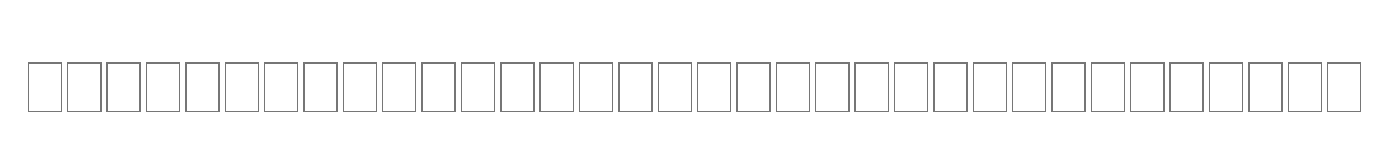
\begin{tikzpicture}
\node[font=\mono\bfseries\fs{13}, text=ink] at (0.25,0.95) {};
\draw[ink!60, line width=0.5pt] (0.04,0) rectangle (0.46,0.62);
\node[font=\mono\bfseries\fs{13}, text=ink] at (0.75,0.95) {};
\draw[ink!60, line width=0.5pt] (0.54,0) rectangle (0.96,0.62);
\node[font=\mono\bfseries\fs{13}, text=ink] at (1.25,0.95) {};
\draw[ink!60, line width=0.5pt] (1.04,0) rectangle (1.46,0.62);
\node[font=\mono\bfseries\fs{13}, text=ink] at (1.75,0.95) {};
\draw[ink!60, line width=0.5pt] (1.54,0) rectangle (1.96,0.62);
\node[font=\mono\bfseries\fs{13}, text=ink] at (2.25,0.95) {};
\draw[ink!60, line width=0.5pt] (2.04,0) rectangle (2.46,0.62);
\node[font=\mono\bfseries\fs{13}, text=ink] at (2.75,0.95) {};
\draw[ink!60, line width=0.5pt] (2.54,0) rectangle (2.96,0.62);
\node[font=\mono\bfseries\fs{13}, text=ink] at (3.25,0.95) {};
\draw[ink!60, line width=0.5pt] (3.04,0) rectangle (3.46,0.62);
\node[font=\mono\bfseries\fs{13}, text=ink] at (3.75,0.95) {};
\draw[ink!60, line width=0.5pt] (3.54,0) rectangle (3.96,0.62);
\node[font=\mono\bfseries\fs{13}, text=ink] at (4.25,0.95) {};
\draw[ink!60, line width=0.5pt] (4.04,0) rectangle (4.46,0.62);
\node[font=\mono\bfseries\fs{13}, text=ink] at (4.75,0.95) {};
\draw[ink!60, line width=0.5pt] (4.54,0) rectangle (4.96,0.62);
\node[font=\mono\bfseries\fs{13}, text=ink] at (5.25,0.95) {};
\draw[ink!60, line width=0.5pt] (5.04,0) rectangle (5.46,0.62);
\node[font=\mono\bfseries\fs{13}, text=ink] at (5.75,0.95) {};
\draw[ink!60, line width=0.5pt] (5.54,0) rectangle (5.96,0.62);
\node[font=\mono\bfseries\fs{13}, text=ink] at (6.25,0.95) {};
\draw[ink!60, line width=0.5pt] (6.04,0) rectangle (6.46,0.62);
\node[font=\mono\bfseries\fs{13}, text=ink] at (6.75,0.95) {};
\draw[ink!60, line width=0.5pt] (6.54,0) rectangle (6.96,0.62);
\node[font=\mono\bfseries\fs{13}, text=ink] at (7.25,0.95) {};
\draw[ink!60, line width=0.5pt] (7.04,0) rectangle (7.46,0.62);
\node[font=\mono\bfseries\fs{13}, text=ink] at (7.75,0.95) {};
\draw[ink!60, line width=0.5pt] (7.54,0) rectangle (7.96,0.62);
\node[font=\mono\bfseries\fs{13}, text=ink] at (8.25,0.95) {};
\draw[ink!60, line width=0.5pt] (8.04,0) rectangle (8.46,0.62);
\node[font=\mono\bfseries\fs{13}, text=ink] at (8.75,0.95) {};
\draw[ink!60, line width=0.5pt] (8.54,0) rectangle (8.96,0.62);
\node[font=\mono\bfseries\fs{13}, text=ink] at (9.25,0.95) {};
\draw[ink!60, line width=0.5pt] (9.04,0) rectangle (9.46,0.62);
\node[font=\mono\bfseries\fs{13}, text=ink] at (9.75,0.95) {};
\draw[ink!60, line width=0.5pt] (9.54,0) rectangle (9.96,0.62);
\node[font=\mono\bfseries\fs{13}, text=ink] at (10.25,0.95) {};
\draw[ink!60, line width=0.5pt] (10.04,0) rectangle (10.46,0.62);
\node[font=\mono\bfseries\fs{13}, text=ink] at (10.75,0.95) {};
\draw[ink!60, line width=0.5pt] (10.54,0) rectangle (10.96,0.62);
\node[font=\mono\bfseries\fs{13}, text=ink] at (11.25,0.95) {};
\draw[ink!60, line width=0.5pt] (11.04,0) rectangle (11.46,0.62);
\node[font=\mono\bfseries\fs{13}, text=ink] at (11.75,0.95) {};
\draw[ink!60, line width=0.5pt] (11.54,0) rectangle (11.96,0.62);
\node[font=\mono\bfseries\fs{13}, text=ink] at (12.25,0.95) {};
\draw[ink!60, line width=0.5pt] (12.04,0) rectangle (12.46,0.62);
\node[font=\mono\bfseries\fs{13}, text=ink] at (12.75,0.95) {};
\draw[ink!60, line width=0.5pt] (12.54,0) rectangle (12.96,0.62);
\node[font=\mono\bfseries\fs{13}, text=ink] at (13.25,0.95) {};
\draw[ink!60, line width=0.5pt] (13.04,0) rectangle (13.46,0.62);
\node[font=\mono\bfseries\fs{13}, text=ink] at (13.75,0.95) {};
\draw[ink!60, line width=0.5pt] (13.54,0) rectangle (13.96,0.62);
\node[font=\mono\bfseries\fs{13}, text=ink] at (14.25,0.95) {};
\draw[ink!60, line width=0.5pt] (14.04,0) rectangle (14.46,0.62);
\node[font=\mono\bfseries\fs{13}, text=ink] at (14.75,0.95) {};
\draw[ink!60, line width=0.5pt] (14.54,0) rectangle (14.96,0.62);
\node[font=\mono\bfseries\fs{13}, text=ink] at (15.25,0.95) {};
\draw[ink!60, line width=0.5pt] (15.04,0) rectangle (15.46,0.62);
\node[font=\mono\bfseries\fs{13}, text=ink] at (15.75,0.95) {};
\draw[ink!60, line width=0.5pt] (15.54,0) rectangle (15.96,0.62);
\node[font=\mono\bfseries\fs{13}, text=ink] at (16.25,0.95) {};
\draw[ink!60, line width=0.5pt] (16.04,0) rectangle (16.46,0.62);
\node[font=\mono\bfseries\fs{13}, text=ink] at (16.75,0.95) {};
\draw[ink!60, line width=0.5pt] (16.54,0) rectangle (16.96,0.62);
\end{tikzpicture}\par

\vfill
\begin{center}
\rotatebox{180}{\parbox{0.95\textwidth}{\fs{8} Lösungen – 1: GUT GEMACHT · 2: MATHE MACHT SPASS · 3: Schlüssel 11, WELCHES TIER SPRINGT HOEHER ALS EIN HAUS JEDES DENN HAEUSER SPRINGEN NIE · 4: MATHE IST EINE GEHEIMWAFFE · 5a: Nichts, jeder Buchstabe läuft einmal im Kreis. 5b: Schlüssel 8. 5c: 26 · 26 = 676.}}
\end{center}

\vspace{2mm}
\blattfuss
\end{document}
